% IT Ethics Lecture 3: Free Speech Online
% Brendan Shea, PhD
% Rochester Community and Technical College

\documentclass[aspectratio=169]{beamer}

% Theme and colors
\usetheme{Madrid}
\usecolortheme{whale}
\setbeamertemplate{navigation symbols}{}
\setbeamertemplate{footline}[frame number]

% Packages
\usepackage[utf8]{inputenc}
\usepackage[T1]{fontenc}
\usepackage{graphicx}
\usepackage{booktabs}
\usepackage{array}
\usepackage{multirow}
\usepackage{hyperref}
\usepackage{csquotes}

% References
\usepackage[backend=biber,style=authoryear]{biblatex}
\addbibresource{refs.bib}

% TikZ and libraries
\usepackage{tikz}
\usetikzlibrary{shapes.geometric, arrows.meta, positioning, calc, backgrounds, fit, decorations.pathreplacing, shadows, mindmap, trees}

% Custom colors
\definecolor{primaryblue}{RGB}{0,74,124}
\definecolor{accentorange}{RGB}{230,126,34}
\definecolor{lightgray}{RGB}{245,245,245}
\definecolor{darktext}{RGB}{44,62,80}


% Title information
\title[IT Ethics: Lecture 3]{Free Speech Online}
\subtitle{Philosophy, Platforms, and Controversy}
\author{Brendan Shea, PhD}
\institute[RCTC]{Rochester Community and Technical College}
\date{}

\begin{document}

%------------------------------------------------------
% SLIDE 1: Title Slide
%------------------------------------------------------
\begin{frame}
\titlepage
\end{frame}

%------------------------------------------------------
% SLIDE 2: What Is Free Speech?
%------------------------------------------------------
\begin{frame}{What Is Free Speech?}
    \begin{itemize}
        \item The term \textbf{freedom of speech} refers to the right to express opinions, ideas, and information without government interference or censorship.
        \item Philosophers often use the broader term \textbf{freedom of expression} to include artistic expression, symbolic acts (such as burning flags or wearing armbands), and other communicative conduct beyond literal speech.
        \item The classic liberal conception treats free speech as a \textbf{negative liberty}, meaning freedom \textit{from} interference by others, especially the state, rather than a positive entitlement to resources or platforms.
        \item Free speech protections vary enormously across legal systems, with the U.S. First Amendment providing unusually strong protections compared to most other democracies.
    \end{itemize}
    
    \vspace{0.3em}
    
    \begin{block}{Key Distinction}
        A \textbf{negative liberty} means the state may not \textit{prevent} you from speaking, while a \textbf{positive liberty} would mean the state must \textit{provide} you with means to speak effectively. Most free speech traditions focus on negative liberty, but online debates increasingly raise positive questions about access to platforms and algorithmic visibility.
    \end{block}
\end{frame}

%------------------------------------------------------
% SLIDE 3: Why Does Free Speech Matter?
%------------------------------------------------------
\begin{frame}{Why Does Free Speech Matter?}
    \begin{itemize}
        \item Speaking our minds is central to who we are, so restricting speech restricts our ability to develop and express our identities---this is the value of \textbf{self-expression}.
        \item Open debate helps us discover truth and correct errors, since no authority is infallible enough to decide what's true for everyone---this is the value of \textbf{truth-seeking}.
        \item Citizens must be able to criticize government, debate policy, and persuade each other for democracy to function, making free speech essential to \textbf{democratic self-governance}.
        \item Free speech and a free press serve as watchdogs against government corruption, abuse, and overreach, providing a crucial mechanism for \textbf{checking power}.
    \end{itemize}
    
    \vspace{0.2em}
    
    \begin{center}
    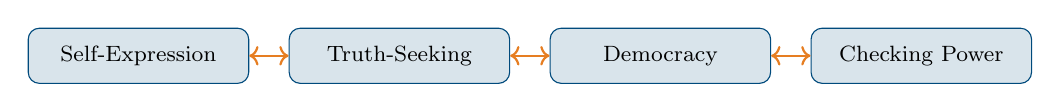
\begin{tikzpicture}[
        node distance=0.8cm,
        value/.style={rectangle, draw=primaryblue, fill=primaryblue!15, rounded corners, minimum width=2.8cm, minimum height=0.7cm, align=center, font=\footnotesize}
    ]
        \node[value] (self) {Self-Expression};
        \node[value, right=0.5cm of self] (truth) {Truth-Seeking};
        \node[value, right=0.5cm of truth] (democracy) {Democracy};
        \node[value, right=0.5cm of democracy] (power) {Checking Power};
        
        \draw[thick, accentorange, <->] (self) -- (truth);
        \draw[thick, accentorange, <->] (truth) -- (democracy);
        \draw[thick, accentorange, <->] (democracy) -- (power);
    \end{tikzpicture}
    \end{center}
\end{frame}

%------------------------------------------------------
% SLIDE 4: Free Speech Online: What's Different?
%------------------------------------------------------
\begin{frame}{Free Speech Online: What's Different?}
    \begin{itemize}
        \item Online speech operates at unprecedented \textbf{scale}, with a single post capable of reaching millions of people instantly without traditional media gatekeepers.
        \item Information and misinformation spread with remarkable \textbf{speed}, often leaving no time for counter-speech or fact-checking before damage is done.
        \item Digital content has a troubling \textbf{permanence}, since posts can be archived, screenshotted, and resurface years later---the internet ``never forgets.''
        \item The possibility of \textbf{anonymity} online enables both valuable whistleblowing and accountability-free harassment.
    \end{itemize}
    
    \begin{center}
    \renewcommand{\arraystretch}{1.1}
    \footnotesize
    \begin{tabular}{>{\raggedright}p{2.5cm} >{\raggedright}p{4.5cm} >{\raggedright\arraybackslash}p{4.5cm}}
        \toprule
        \textbf{Feature} & \textbf{Traditional Media} & \textbf{Online Speech} \\
        \midrule
        Distribution & Gatekeepers (editors, publishers) & Anyone can publish instantly \\
        Reach & Local or national audiences & Global, potentially viral \\
        Accountability & Authors typically known & Often anonymous \\
        Duration & Yesterday's news & Archived indefinitely \\
        Amplification & Editorial judgment & Algorithmic optimization \\
        \bottomrule
    \end{tabular}
    \end{center}
\end{frame}

%------------------------------------------------------
% SLIDE 5: Mill's Harm Principle
%------------------------------------------------------
\begin{frame}{Mill's Harm Principle}
    \begin{itemize}
        \item The philosopher John Stuart Mill articulated the most influential liberal framework for free speech in his 1859 work \textit{On Liberty} \parencite*{mill1859liberty}.
        \item Mill's \textbf{harm principle} holds that the only legitimate reason for society to restrict an individual's liberty is to prevent harm to others---not to protect the individual from themselves or to enforce moral conformity.
        \item According to Mill, the fact that others find your speech offensive, immoral, or wrong is never sufficient justification for silencing you.
        \item This principle places the \textbf{burden of proof} on those who would restrict speech: they must demonstrate that the speech causes genuine harm to others, not merely that it is disagreeable or unpopular.
    \end{itemize}
    
    \vspace{0.3em}
    
    \begin{block}{Mill, \textit{On Liberty} (1859)}
        ``The only purpose for which power can be rightfully exercised over any member of a civilized community, against his will, is to prevent harm to others. His own good, either physical or moral, is not a sufficient warrant.''
    \end{block}
\end{frame}

%------------------------------------------------------
% SLIDE 6: Mill's Marketplace of Ideas
%------------------------------------------------------
\begin{frame}{Mill's Marketplace of Ideas}
    \begin{itemize}
        \item Mill argues that open debate is the best method for discovering truth, since no authority---whether government, church, or majority opinion---is infallible enough to decide what is true for everyone.
        \item Even opinions that seem obviously false should be permitted, because the process of refuting them helps us better understand \textit{why} they are false and strengthens our grasp of the truth.
        \item Mill warns that beliefs held without challenge become ``dead dogma''---we mouth the words but lose genuine understanding of their meaning and justification.
        \item This argument is often called the \textbf{marketplace of ideas}: just as economic competition produces better products, intellectual competition produces better ideas.
    \end{itemize}
    
    \vspace{0.3em}
    
    \begin{alertblock}{Mill's Fallibilism}
        Mill's argument rests on \textbf{fallibilism}---the recognition that any of our beliefs might be wrong. If we silence dissent, we lose the opportunity to correct our errors. Even if the silenced opinion is false, we lose the ``clearer perception and livelier impression of truth, produced by its collision with error.''
    \end{alertblock}
\end{frame}

%------------------------------------------------------
% SLIDE 7: Mill's Listener Autonomy
%------------------------------------------------------
\begin{frame}{Mill's Listener Autonomy}
    \begin{itemize}
        \item Mill's defense of free speech emphasizes not just the rights of speakers but the rights of \textbf{listeners} to hear and evaluate ideas for themselves.
        \item When the state censors speech to ``protect'' citizens from dangerous or false ideas, it treats adults like children who cannot be trusted to think for themselves.
        \item Respecting \textbf{listener autonomy} means allowing people access to the full range of opinions and arguments so they can make up their own minds.
        \item This argument suggests that censorship is paternalistic: it assumes the government knows better than citizens what ideas they should encounter.
    \end{itemize}
    
    \vspace{0.3em}
    
    \begin{exampleblock}{The Paternalism Objection}
        Imagine a government that bans books arguing for atheism because it believes religious faith is good for citizens. Even if the government is right that faith is beneficial, Mill would argue this censorship wrongs citizens by denying them the opportunity to consider the arguments and decide for themselves.
    \end{exampleblock}
\end{frame}

%------------------------------------------------------
% SLIDE 8: Applying Mill: When Is Restriction Justified?
%------------------------------------------------------
\begin{frame}{Applying Mill: When Is Restriction Justified?}
    \small
    \begin{itemize}
        \item Mill does not believe free speech is absolute---speech that directly causes harm to others can be restricted under the harm principle.
        \item Mill's famous example involves a corn dealer: writing that corn dealers starve the poor is protected speech, but shouting the same words to an angry mob outside a corn dealer's house may be punished.
        \item The key distinction is whether there is time for \textbf{counter-speech}---if the harm is imminent and there's no opportunity for debate, restriction may be justified.
        \item Mill thus establishes a high bar: restriction requires not just potential harm, but harm that is direct, imminent, and unavoidable through further discussion.
    \end{itemize}
    
    \vspace{0.2em}
    
    \begin{center}
    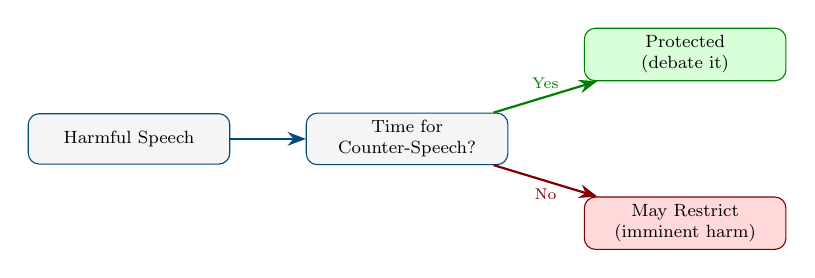
\begin{tikzpicture}[
        scale=.8,
        transform shape,
        node distance=1.5cm,
        box/.style={rectangle, draw=primaryblue, fill=lightgray, rounded corners, minimum width=3.2cm, minimum height=0.8cm, align=center, font=\footnotesize}
    ]
        \node[box] (speech) {Harmful Speech};
        \node[box, right=1.2cm of speech] (time) {Time for\\Counter-Speech?};
        \node[box, above right=0.5cm and 1.2cm of time, fill=green!15, draw=green!50!black] (protect) {Protected\\(debate it)};
        \node[box, below right=0.5cm and 1.2cm of time, fill=red!15, draw=red!50!black] (restrict) {May Restrict\\(imminent harm)};
        
        \draw[-{Stealth}, thick, primaryblue] (speech) -- (time);
        \draw[-{Stealth}, thick, green!50!black] (time) -- node[above, font=\scriptsize] {Yes} (protect);
        \draw[-{Stealth}, thick, red!50!black] (time) -- node[below, font=\scriptsize] {No} (restrict);
    \end{tikzpicture}
    \end{center}
\end{frame}

%------------------------------------------------------
% SLIDE 9: The Rawls/Dworkin Approach: A Different Foundation
%------------------------------------------------------
\begin{frame}{The Rawls/Dworkin Approach: A Different Foundation}
    \begin{itemize}
        \item Philosophers John Rawls \parencite*{rawls1971theory, rawls1993political} and Ronald Dworkin \parencite*{dworkin1996freedoms} offer a different justification for free speech that focuses on \textbf{equal dignity and respect} rather than on the good consequences of open debate.
        \item While Mill's argument is \textbf{consequentialist}---free speech is valuable because it produces good outcomes like truth and progress---the Rawls/Dworkin approach is \textbf{rights-based}.
        \item On this view, free speech is not just useful; it is \textit{required} by the basic moral principle that all persons deserve equal respect as autonomous agents capable of forming their own views.
        \item This means free speech protections don't depend on proving that the ``marketplace of ideas'' actually works---they follow directly from respecting persons as equals.
    \end{itemize}
    
    \vspace{0.3em}
    
    \begin{block}{Two Different Questions}
        Mill asks: ``Does free speech produce good results?'' Rawls and Dworkin ask: ``What does treating citizens as free and equal require?'' Both answers support free speech, but for fundamentally different reasons.
    \end{block}
\end{frame}

%------------------------------------------------------
% SLIDE 10: Dworkin's Moral Independence
%------------------------------------------------------
\begin{frame}{Dworkin's Moral Independence}
    \begin{itemize}
        \item Ronald Dworkin argues that individuals have a right to \textbf{moral independence}---the right not to be disadvantaged simply because others disapprove of their opinions or way of life.
        \item According to Dworkin, the fact that a majority finds your views offensive, immoral, or worthless is never a legitimate reason for the state to silence you.
        \item This is because allowing majorities to suppress minority views based on moral disapproval violates the fundamental principle that all citizens must be treated with \textbf{equal concern and respect}.
        \item Dworkin's argument protects even deeply unpopular speech: the Nazis' right to march, the racist's right to speak, the pornographer's right to publish---not because their views have value, but because silencing them based on disapproval treats them as less than equal citizens.
    \end{itemize}
    
    \vspace{0.3em}
    
    \begin{alertblock}{The Hard Cases}
        Dworkin's view is most controversial precisely where it matters most: protecting speech that most people find abhorrent. The test of a free speech principle, he argues, is whether it protects speech we hate, not speech we like.
    \end{alertblock}
\end{frame}

%------------------------------------------------------
% SLIDE 11: The Legitimacy Argument
%------------------------------------------------------
\begin{frame}{The Legitimacy Argument}
    \begin{itemize}
        \item Rawls and Dworkin also offer a \textbf{legitimacy argument} for free speech that connects it directly to the foundations of democratic government.
        \item Laws are only legitimate---only morally binding on citizens---if those citizens had a fair opportunity to speak against them before they were enacted.
        \item If the government can silence critics before a law is passed, then those who opposed the law cannot be said to have consented to it, even implicitly.
        \item Free speech is thus not just one right among many but a \textbf{precondition of democratic legitimacy} itself---without it, the entire system of laws loses its moral authority.
    \end{itemize}
    
    \vspace{0.3em}
    
    \begin{exampleblock}{Dworkin on Legitimacy}
        Dworkin argues that we cannot legitimately punish someone for violating a law if they were forbidden from arguing against that law before it was passed. Free speech is what makes democratic lawmaking genuinely democratic rather than mere majority tyranny.
    \end{exampleblock}
\end{frame}

%------------------------------------------------------
% SLIDE 12: Discussion Questions: Philosophical Foundations
%------------------------------------------------------
\begin{frame}{Discussion Questions: Philosophical Foundations}
    \begin{enumerate}
        \item Mill argues that even false and harmful opinions should generally be permitted because refuting them strengthens our understanding of truth. Do you find this convincing? Can you think of cases where exposure to false ideas makes people \textit{less} able to recognize truth?
        
        \vspace{0.5em}
        
        \item Dworkin claims that protecting speech we find abhorrent is the real test of commitment to free speech. Is there any speech so harmful that this principle should not apply? Where would you draw the line?
        
        \vspace{0.5em}
        
        \item The legitimacy argument says laws are only binding if citizens could speak against them. Does this apply to social media platform rules, which users had no voice in creating? Should it?
        
        \vspace{0.5em}
        
        \item Mill wrote before the internet existed. Does the unprecedented scale and speed of online speech change his arguments? Is there still ``time for counter-speech'' when misinformation goes viral in minutes?
    \end{enumerate}
\end{frame}

%------------------------------------------------------
% SLIDE 13: What Is Hate Speech?
%------------------------------------------------------
\begin{frame}{What Is Hate Speech?}
    \begin{itemize}
        \item \textbf{Hate speech} refers to expression that attacks, demeans, or incites violence against people based on characteristics such as race, ethnicity, religion, gender, sexual orientation, or disability.
        \item Hate speech exists on a spectrum from crude slurs and stereotypes to sophisticated ideological arguments for the inferiority or dangerousness of certain groups.
        \item The term is contested: some argue it is too vague to regulate fairly, while others insist that the harms it causes are clear enough to justify legal restrictions.
        \item Online platforms have dramatically amplified hate speech by enabling anonymous posting, algorithmic promotion of inflammatory content, and the formation of extremist communities across geographic boundaries.
    \end{itemize}
    
    \vspace{0.3em}
    
    \begin{block}{The Spectrum of Hate Speech}
        Not all hate speech is equally harmful or equally easy to identify. Explicit calls for violence (``Kill all X'') differ from dehumanizing rhetoric (``X are animals''), which differs from coded language and ``dog whistles'' that signal hateful views to insiders while maintaining plausible deniability.
    \end{block}
\end{frame}

%------------------------------------------------------
% REVISED SLIDE 14: The Case for Restricting Hate Speech
% Changed: alertblock → table of harm types
%------------------------------------------------------
\begin{frame}{The Case for Restricting Hate Speech}
    \begin{itemize}
        \item Defenders of hate speech restrictions argue that such speech causes serious \textbf{dignitary harm} by denying the equal moral standing of targeted groups.
        \item Philosopher Jeremy Waldron \parencite*{waldron2012} argues that hate speech functions as \textbf{group defamation}---undermining the public assurance of equal citizenship.
        \item Perhaps most seriously, hate speech may lead to \textbf{physical violence} by normalizing hatred and dehumanizing targets---a pattern visible in genocides from the Holocaust to Rwanda.
    \end{itemize}
    
    \vspace{0.5em}
    
    \begin{table}[h]
        \centering
        \small
        \begin{tabular}{|l|l|l|}
            \hline
            \textbf{Type of Harm} & \textbf{Mechanism} & \textbf{Example} \\
            \hline
            Dignitary & Denies equal standing & Slurs, dehumanization \\
            Psychological & Trauma, anxiety, depression & Sustained harassment \\
            Silencing & Intimidates targets into silence & Threats, doxxing \\
            Physical & Incites or justifies violence & Genocide propaganda \\
            \hline
        \end{tabular}
    \end{table}
\end{frame}
%------------------------------------------------------
% SLIDE 15: The Case Against Restricting Hate Speech
%------------------------------------------------------
\begin{frame}{The Case Against Restricting Hate Speech}
    \begin{itemize}
        \item Critics of hate speech laws argue that the concept is too \textbf{vague and subjective} to regulate fairly---what counts as ``hateful'' depends heavily on who is making the judgment and their political perspective.
        \item History shows that speech restrictions are often \textbf{used against the marginalized} they are meant to protect: early hate speech prosecutions in the U.S. targeted civil rights activists, and blasphemy laws worldwide are used to persecute religious minorities.
        \item Following Mill, some argue that \textbf{counter-speech is more effective} than censorship---driving hateful views underground may make them harder to monitor and refute, while public exposure allows them to be challenged.
    \end{itemize}    
    \vspace{0.3em}
    
    \begin{exampleblock}{The Slippery Slope Concern}
        Who decides what counts as hate speech? Today's protected minority may become tomorrow's majority with the power to silence critics. Many free speech advocates worry that hate speech laws inevitably expand beyond their original targets.
    \end{exampleblock}
\end{frame}

%------------------------------------------------------
% SLIDE 16: Case Study: Charlottesville and Online Radicalization (2017)
%------------------------------------------------------
\begin{frame}{Case Study: Charlottesville and Online Radicalization (2017)}
    \small
    \begin{itemize}
        \item In August 2017, white supremacists organized the ``Unite the Right'' rally in Charlottesville, Virginia, where counter-protester Heather Heyer was killed when a participant drove his car into a crowd.
        \item The rally was organized primarily through online platforms including Discord, Reddit, and 4chan, which allowed geographically dispersed extremists to coordinate and recruit new members.
        \item Investigators found that the attacker, James Alex Fields Jr., had been radicalized through online exposure to white supremacist content, following a pattern researchers call the \textbf{radicalization pipeline}.
        \item After Charlottesville, major platforms including Discord, GoDaddy, and Cloudflare took unprecedented steps to ban extremist groups, sparking debate about whether \textbf{deplatforming} reduces harm or simply pushes extremists to less visible corners of the internet.
    \end{itemize}
    
    \vspace{0.3em}
    
    \begin{block}{Key Question}
        \scriptsize
        Should platforms be held responsible for hosting content that contributes to real-world violence? Or does holding them responsible create dangerous incentives to over-censor?
    \end{block}
\end{frame}

%------------------------------------------------------
% SLIDE 17: Case Study: Christchurch and Livestreamed Violence (2019)
%------------------------------------------------------
\begin{frame}{Case Study: Christchurch and Livestreamed Violence (2019)}
    \small
    \begin{itemize}
        \item On March 15, 2019, a gunman attacked two mosques in Christchurch, New Zealand, killing 51 people---while livestreaming the massacre on Facebook Live to an audience that initially numbered in the dozens but quickly grew.
        \item The attacker had posted a manifesto on 8chan filled with white supremacist ideology and internet memes, illustrating how online extremist communities blend serious radicalization with ironic humor to recruit young people.
        \item Facebook reported that in the first 24 hours, users attempted to upload the video 1.5 million times, with 1.2 million blocked at upload---but 300,000 copies still got through and spread across platforms.
        \item The attack prompted the \textbf{Christchurch Call}, an international agreement between governments and tech companies to eliminate terrorist and violent extremist content online, raising questions about global internet governance.
    \end{itemize}
    
    \vspace{0.3em}
    
    \begin{alertblock}{The Virality Problem}
        \small
        Traditional media would never broadcast a mass shooting in real time. But social media's design---optimized for engagement and sharing---can turn atrocities into viral content before human moderators can respond.
    \end{alertblock}
\end{frame}

%------------------------------------------------------
% SLIDE 18: Case Study: Gamergate and Coordinated Harassment (2014)
%------------------------------------------------------
\begin{frame}{Case Study: Gamergate and Coordinated Harassment (2014)}
    \begin{itemize}
        \small
        \item \textbf{Gamergate} began in 2014 as an online harassment campaign targeting women in the video game industry, including developer Zoe Quinn and cultural critic Anita Sarkeesian, who received death threats, rape threats, and had their personal information published online.
        \item Participants claimed to be concerned about ``ethics in gaming journalism,'' but researchers found the movement functioned primarily as coordinated harassment, with anonymous users organizing attacks through platforms like 4chan, Reddit, and Twitter.
        \item Targets faced \textbf{doxxing} (publication of home addresses and phone numbers), \textbf{swatting} (false reports to police designed to trigger armed responses), and sustained campaigns that forced some to flee their homes.
        \item Gamergate is now recognized as a template for later online harassment campaigns and as a \textbf{gateway to broader far-right radicalization}, with many participants later becoming active in white nationalist movements.
    \end{itemize}
    
    \vspace{0.3em}
    
    \begin{block}{Harassment as Silencing}
        \small
        Several Gamergate targets left the gaming industry or reduced their public presence. This illustrates how coordinated harassment can function as a form of censorship---silencing speakers not through law but through fear.
    \end{block}
\end{frame}

%------------------------------------------------------
% SLIDE 19: Deplatforming: The Case of Alex Jones (2018)
%------------------------------------------------------
\begin{frame}{Deplatforming: The Case of Alex Jones (2018)}
    \begin{itemize}
        \item Alex Jones, host of the conspiracy theory website InfoWars, was banned from Facebook, YouTube, Apple, and Spotify in August 2018 for repeatedly violating policies against hate speech and harassment.
        \item Jones had promoted false claims that the 2012 Sandy Hook school shooting was a hoax and that grieving parents were ``crisis actors''---claims that led his followers to harass and threaten the families of murdered children.
        \item Research after his deplatforming found that mentions of Jones and InfoWars across social media \textbf{dropped by 50\%}, and his ability to reach new audiences was dramatically reduced.
        \item Critics argued that coordinated deplatforming by major tech companies represented dangerous corporate censorship, while supporters contended that private companies have no obligation to amplify harmful content.
    \end{itemize}
    
    \vspace{0.3em}
    
    \begin{exampleblock}{Does Deplatforming Work?}
        Studies suggest deplatforming reduces reach and recruitment for extremists. But it doesn't change minds---Jones retained his core audience on alternative platforms. The debate is whether reducing amplification is enough.
    \end{exampleblock}
\end{frame}

%------------------------------------------------------
% SLIDE 20: Deplatforming: The Case of Donald Trump (2021)
%------------------------------------------------------
\begin{frame}{Deplatforming: The Case of Donald Trump (2021)}
    \begin{itemize}
        \item On January 8, 2021---two days after the Capitol riot---Twitter permanently suspended President Donald Trump's account, citing ``the risk of further incitement of violence''; Facebook, YouTube, and other platforms followed.
        \item The decision was unprecedented: a sitting U.S. president, with 88 million Twitter followers, was removed from the platforms that had defined his political communication style.
        \item Supporters of the ban argued Trump had used social media to spread election fraud claims that directly incited the January 6th attack; critics argued that unelected tech executives should not have the power to silence elected leaders.
        \item The incident intensified debates about \textbf{platform power}: if social media companies can ban a president, what limits exist on their control over public discourse?
    \end{itemize}
    
    \vspace{0.3em}
    
    \begin{block}{A Question of Power}
        German Chancellor Angela Merkel, no ally of Trump, called the ban ``problematic,'' arguing that the rules governing political speech should be set by legislators, not corporate terms of service. Who \textit{should} make these decisions?
    \end{block}
\end{frame}

%------------------------------------------------------
% SLIDE 21: International Approaches to Hate Speech
%------------------------------------------------------
\begin{frame}{International Approaches to Hate Speech}
    \begin{itemize}
        \item The United States has the world's strongest legal protections for hate speech, with the First Amendment generally protecting even explicitly racist and hateful expression unless it constitutes a direct incitement to imminent violence.
        \item Most European democracies take a different approach: Germany's \textbf{NetzDG law} (2017) requires platforms to remove ``manifestly unlawful'' hate speech within 24 hours or face fines up to 50 million euros.
        \item The European Union's \textbf{Digital Services Act} (2022) creates continent-wide obligations for platforms to address illegal content, including hate speech, with significant penalties for non-compliance.
        \item This creates a patchwork: content legal in the U.S. may be illegal in Germany, forcing global platforms to make difficult decisions about whether to apply the strictest standard everywhere or customize content by region.
    \end{itemize}
    
    \vspace{0.3em}
    
    \begin{table}[h]
        \centering
        \scriptsize
        \begin{tabular}{|l|c|c|}
            \hline
            \textbf{Country/Region} & \textbf{Hate Speech Laws?} & \textbf{Holocaust Denial Illegal?} \\
            \hline
            United States & Limited & No \\
            Germany & Yes & Yes \\
            France & Yes & Yes \\
            United Kingdom & Yes & No \\
            \hline
        \end{tabular}
    \end{table}
\end{frame}

%------------------------------------------------------
% SLIDE 22: The Amplification Problem
%------------------------------------------------------
\begin{frame}{The Amplification Problem}
    \begin{itemize}
        \item Social media platforms don't just host speech---they actively \textbf{amplify} it through algorithmic recommendations, trending topics, and engagement-based ranking that prioritizes content likely to generate strong reactions.
        \item Research has consistently found that inflammatory, outrageous, and divisive content generates more engagement than measured, nuanced content---meaning platform algorithms systematically boost the most extreme voices.
        \item A 2021 internal Facebook study (leaked by whistleblower Frances Haugen) found that the platform's algorithms were ``ichrome exploiting the human brain's attraction to divisiveness'' and that changes to increase engagement had made the platform angrier.
        \item This means that even if platforms don't \textit{create} hate speech, their design choices actively \textbf{spread it further and faster} than would occur through organic sharing alone.
    \end{itemize}
    
    \vspace{0.3em}
    
    \begin{alertblock}{Beyond Neutrality}
        Platforms often claim to be neutral hosts of user content. But algorithmic amplification means they are actively making editorial choices about what speech to promote---even if those choices are made by software rather than humans.
    \end{alertblock}
\end{frame}

%------------------------------------------------------
% REVISED SLIDE 23: Stochastic Terrorism
% Changed: exampleblock → TikZ diagram showing probability and scale
%------------------------------------------------------
\begin{frame}{Stochastic Terrorism}
    \begin{itemize}
        \item \textbf{Stochastic terrorism} refers to using mass media to incite random acts of violence that are statistically predictable but individually unpredictable.
        \item The speaker doesn't direct specific attacks but creates conditions where attacks become likely, while maintaining plausible deniability.
        \item Critics argue the concept is too broad; defenders point to attacks from Pittsburgh (2018) to El Paso (2019) to Buffalo (2022).
    \end{itemize}
    
    \vspace{0.3em}
    
    \centering
    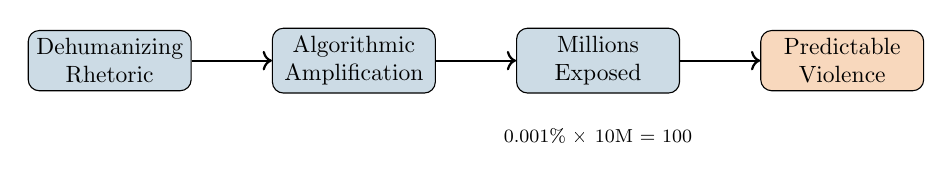
\begin{tikzpicture}[node distance=1.2cm, auto, scale=0.85, transform shape]
        \node[draw, rounded corners, fill=primaryblue!20, text width=2.2cm, align=center] (rhetoric) {Dehumanizing\\Rhetoric};
        \node[draw, rounded corners, fill=primaryblue!20, text width=2.2cm, align=center, right=of rhetoric] (amplify) {Algorithmic\\Amplification};
        \node[draw, rounded corners, fill=primaryblue!20, text width=2.2cm, align=center, right=of amplify] (millions) {Millions\\Exposed};
        \node[draw, rounded corners, fill=accentorange!30, text width=2.2cm, align=center, right=of millions] (violence) {Predictable\\Violence};
        
        \draw[->, thick] (rhetoric) -- (amplify);
        \draw[->, thick] (amplify) -- (millions);
        \draw[->, thick] (millions) -- (violence);
        
        \node[below=0.4cm of millions, text width=3cm, align=center, font=\footnotesize] {0.001\% × 10M = 100};
    \end{tikzpicture}
\end{frame}

%------------------------------------------------------
% SLIDE 24: Discussion Questions: Hate Speech Online
%------------------------------------------------------
\begin{frame}{Discussion Questions: Hate Speech Online}
    \begin{enumerate}
        \item The U.S. protects hate speech that would be illegal in Germany or France. Which approach do you find more persuasive? Does the internet---which crosses all borders---require a global standard?
        
        \vspace{0.5em}
        
        \item Deplatforming Alex Jones reduced his reach by 50\%. Is that a success (less exposure to harmful content) or a failure (he still has an audience and now claims persecution)? What would ``success'' look like?
        
        \vspace{0.5em}
        
        \item If platform algorithms amplify hate speech because it generates engagement, are platforms morally responsible for the content they promote? Should they be legally liable?
        
        \vspace{0.5em}
        
        \item Consider the concept of stochastic terrorism. At what point does inflammatory rhetoric become morally equivalent to incitement, even without explicit calls for violence? How would you draw that line?
    \end{enumerate}
\end{frame}

%------------------------------------------------------
% SLIDE 25: The Traditional Debate Over Pornography
%------------------------------------------------------
\begin{frame}{The Traditional Debate Over Pornography}
    \begin{itemize}
        \small
        \item For most of the 20th century, debates over pornography pitted \textbf{conservative moralists} against \textbf{liberal defenders of free expression}, with conservatives arguing that sexually explicit material corrupts morals and undermines social values.
        \item Liberals responded with arguments drawn from Mill: adults have the right to consume whatever content they choose, and the state should not impose majoritarian moral views on private behavior that harms no one else.
        \item U.S. law developed the \textbf{obscenity doctrine}, which holds that ``obscene'' material is not protected speech---but defining obscenity proved notoriously difficult, leading Justice Potter Stewart to famously write, ``I know it when I see it.''
        \item The internet transformed this debate entirely: pornography went from something purchased in specialized shops to content available instantly, freely, and anonymously to anyone with a smartphone---including children.
    \end{itemize}
    
    \vspace{0.3em}
    
    \begin{block}{The Scale of Online Pornography}
        Pornhub alone reported 42 billion visits in 2019---an average of 115 million per day. The internet has made pornography one of the most consumed forms of media in human history, fundamentally changing the stakes of the debate.
    \end{block}
\end{frame}

%------------------------------------------------------
% REVISED SLIDE 26: MacKinnon's Feminist Critique
% Changed: alertblock → direct quote from MacKinnon
%------------------------------------------------------
\begin{frame}{MacKinnon's Feminist Critique}
    \begin{itemize}
        \item Legal scholar \textbf{Catharine MacKinnon} \parencite*{mackinnon1987feminism, mackinnon1989toward, mackinnon1993only} reframed the pornography debate by arguing that the real harm is not moral corruption but \textbf{the subordination of women}.
        \item MacKinnon argues that pornography functions as a \textbf{speech act}: it doesn't merely express ideas about women but actually \textit{does} something---it defines them as objects existing for male pleasure.
        \item On this view, pornography \textbf{silences women} by shaping how their speech is heard: when a woman says ``no,'' pornography has trained viewers to interpret refusal as part of a sexual script.
        \item This challenges the liberal framework directly: if pornography itself causes harm and silencing, then restricting it doesn't limit free speech---it \textit{enables} speech.
    \end{itemize}
    
    \vspace{0.3em}
    
    \begin{quote}
        \footnotesize
        ``Pornography, in the feminist view, is a form of forced sex... an institution of gender inequality.'' \\ \hfill ---Catharine MacKinnon
    \end{quote}
\end{frame}


%------------------------------------------------------
% SLIDE 27: Case Study: Revenge Porn and Non-Consensual Intimate Images
%------------------------------------------------------
\begin{frame}{Case Study: Revenge Porn and Non-Consensual Intimate Images}
    \begin{itemize}
        \item \textbf{Revenge porn}---more accurately called \textbf{non-consensual intimate images (NCII)}---refers to the distribution of sexually explicit images without the subject's consent, often by former partners seeking to humiliate or control victims.
        \item The harms are severe and well-documented: victims report job loss, relationship destruction, depression, anxiety, and suicide attempts; the images often cannot be fully removed once they spread online.
        \item As of 2024, 48 U.S. states have laws against NCII, though enforcement remains difficult; the federal SHIELD Act (proposed but not yet passed) would create nationwide criminal penalties.
        \item Dedicated websites that host NCII have faced legal action, but content often migrates to mainstream platforms, file-sharing services, and international sites beyond U.S. jurisdiction.
    \end{itemize}
    
    \vspace{0.3em}
    
    \begin{exampleblock}{Consent Is Not Transferable}
        A person may consent to being photographed intimately, or even to sharing images with a partner---but that consent does not extend to public distribution. The violation lies in the distribution, not the creation, of the images.
    \end{exampleblock}
\end{frame}

%------------------------------------------------------
% SLIDE 28: Case Study: Deepfakes and AI-Generated Intimate Images
%------------------------------------------------------
\begin{frame}{Case Study: Deepfakes and AI-Generated Intimate Images}
    \begin{itemize}
        \small
        \item \textbf{Deepfakes} are AI-generated synthetic media that can place anyone's face onto explicit content, creating realistic fake pornography of people who never consented to or participated in such content.
        \item In January 2024, AI-generated explicit images of Taylor Swift went viral on X (formerly Twitter), viewed tens of millions of times before the platform could remove them---illustrating how quickly such content can spread.
        \item While celebrities have resources to fight back, ordinary people---especially women and girls---are increasingly targeted; a 2023 study found that 96\% of deepfake videos online are non-consensual pornography, and the vast majority target women.
        \item Deepfakes represent a new category of harm: the victim never took the photos, never consented to anything, yet faces the same devastating consequences as traditional revenge porn victims.
    \end{itemize}
    
    \vspace{0.3em}
    
    \begin{block}{The Democratization of Harm}
        Creating convincing deepfakes once required significant technical skill. Today, free apps and websites allow anyone to generate explicit fake images in minutes. The barrier to creating this content has essentially disappeared.
    \end{block}
\end{frame}

%------------------------------------------------------
% SLIDE 29: Case Study: OnlyFans and Creator-Controlled Content
%------------------------------------------------------
\begin{frame}{Case Study: OnlyFans and Creator-Controlled Content}
    \begin{itemize}

        \item \textbf{OnlyFans}, launched in 2016, allows creators to sell content directly to subscribers, with the platform taking a 20\% cut---it became famous primarily as a platform for sexual content created and controlled by the performers themselves.
        \item Supporters argue OnlyFans represents a \textbf{feminist alternative} to traditional pornography: creators control their own content, set their own boundaries, keep most of their earnings, and interact directly with their audience without exploitative intermediaries.
        \item Critics raise concerns about \textbf{economic coercion}: when young people turn to OnlyFans due to student debt, low wages, or pandemic job losses, is their ``choice'' truly free? And what are the long-term consequences of permanent online sexual content?
    \end{itemize}
    
    \vspace{0.3em}
    
    \begin{block}{The Autonomy Question}
        OnlyFans forces us to ask what genuine sexual autonomy looks like. Is it enough that creators technically ``choose'' to participate? Or does meaningful autonomy require economic alternatives and full understanding of consequences?
    \end{block}
\end{frame}

%------------------------------------------------------
% SLIDE 30: Children and Online Pornography
%------------------------------------------------------
\begin{frame}{Children and Online Pornography}
    \small
    \begin{itemize}
        \item Unlike previous generations, today's children encounter online pornography not through deliberate seeking but through \textbf{accidental exposure}---pop-up ads, mislabeled content, social media links, and peer sharing on school devices.
        \item Research suggests the average age of first exposure to online pornography is between 11 and 13, with many children encountering explicit content even younger; most have seen pornography before receiving any formal sex education.
        \item Concerns focus on pornography's potential to shape developing attitudes about sex, consent, and relationships---particularly given that mainstream online pornography frequently depicts aggression, lack of consent communication, and unrealistic body standards.
        \item Age verification systems remain controversial: effective verification requires collecting personal data (raising privacy concerns), while ineffective systems are easily bypassed by tech-savvy children.
    \end{itemize}
    
    \vspace{0.3em}
    
    \begin{alertblock}{A Different Harm Calculus}
        Mill's harm principle assumes autonomous adults capable of evaluating information for themselves. Children's developing brains and lack of context change the ethical calculation---most agree that protecting children justifies restrictions that would be inappropriate for adults.
    \end{alertblock}
\end{frame}

%------------------------------------------------------
% SLIDE 31: Consent in the Digital Age
%------------------------------------------------------
\begin{frame}{Consent in the Digital Age}
    \begin{itemize}
        \item The internet has complicated \textbf{consent} in ways that earlier free speech frameworks never anticipated: content can be copied, shared, and preserved indefinitely without the subject's ongoing agreement.
        \item A person may consent to creating intimate content at one point in their life, but that content can resurface decades later in entirely different contexts---can consent given at 19 bind someone at 40?
        \item The question of \textbf{informed consent} becomes especially fraught when young people may not fully understand how permanent digital content is, how widely it may spread, or how it may affect future employment, relationships, and opportunities.
    \end{itemize}
    
    \vspace{0.3em}
    
    \begin{exampleblock}{The Right to Be Forgotten}
        Some European courts have recognized a ``right to be forgotten''---the ability to have past information delisted from search results. Should this right extend to sexual content? Can someone withdraw consent years later?
    \end{exampleblock}
\end{frame}

%------------------------------------------------------
% SLIDE 32: Discussion Questions: Pornography and Sexual Content Online
%------------------------------------------------------
\begin{frame}{Discussion Questions: Pornography and Sexual Content Online}
    \begin{enumerate}
        \item MacKinnon argues that pornography silences women by changing how their speech is interpreted. Do you find this argument convincing? How would you test whether it's true?
        
        \vspace{0.5em}
        
        \item Should AI-generated deepfake pornography be treated the same as ``real'' non-consensual intimate images, even though no actual sexual act occurred? What is the nature of the harm?
        
        \vspace{0.5em}
        
        \item OnlyFans creators choose to participate and control their own content. Is this genuine empowerment, or does economic pressure undermine meaningful consent? Where do you draw the line?
        
        \vspace{0.5em}
        
        \item Most agree children should be protected from pornography. But age verification requires collecting personal data. How do we balance protecting children against privacy concerns for adults?
    \end{enumerate}
\end{frame}

%------------------------------------------------------
% REVISED SLIDE 33: What Is Cancel Culture?
% Changed: block → spectrum diagram
%------------------------------------------------------
\begin{frame}{What Is Cancel Culture?}
    \begin{itemize}
        \item \textbf{Cancel culture} refers to withdrawing support from public figures after objectionable speech or behavior---often through organized social media campaigns.
        \item Defenders argue cancellation is simply \textbf{accountability}---marginalized groups using collective action to impose consequences on the powerful.
        \item Critics argue it creates a \textbf{climate of fear}, with punishments often disproportionate and lacking due process.
    \end{itemize}
    
    \vspace{0.3em}
    
    \centering
    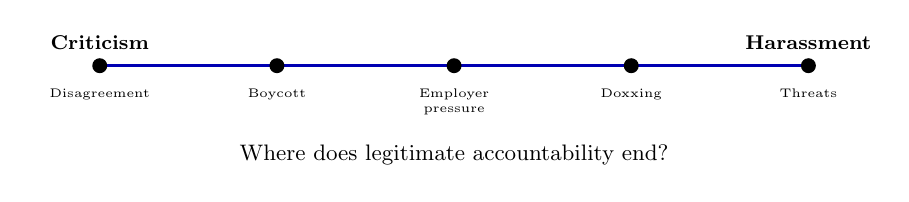
\begin{tikzpicture}[scale=0.9, transform shape]
        % Spectrum line
        \draw[very thick, blue!70!black] (0,0) -- (10,0);
        
        % Endpoints
        \node[above] at (0,0.1) {\footnotesize\textbf{Criticism}};
        \node[above] at (10,0.1) {\footnotesize\textbf{Harassment}};
        
        % Markers
        \fill (0,0) circle (3pt);
        \node[below, text width=1.8cm, align=center, font=\tiny] at (0,-0.2) {Disagreement};
        \fill (2.5,0) circle (3pt);
        \node[below, text width=1.8cm, align=center, font=\tiny] at (2.5,-0.2) {Boycott};
        \fill (5,0) circle (3pt);
        \node[below, text width=1.8cm, align=center, font=\tiny] at (5,-0.2) {Employer pressure};
        \fill (7.5,0) circle (3pt);
        \node[below, text width=1.8cm, align=center, font=\tiny] at (7.5,-0.2) {Doxxing};
        \fill (10,0) circle (3pt);
        \node[below, text width=1.8cm, align=center, font=\tiny] at (10,-0.2) {Threats};
        
        % Question
        \node[below] at (5,-1) {\small Where does legitimate accountability end?};
    \end{tikzpicture}
\end{frame}

%------------------------------------------------------
% SLIDE 34: Case Study: Justine Sacco (2013)
%------------------------------------------------------
\begin{frame}{Case Study: Justine Sacco (2013)}
    \begin{itemize}
        \item In December 2013, Justine Sacco, a PR executive with 170 Twitter followers, posted a tweet before boarding a flight to South Africa: ``Going to Africa. Hope I don't get AIDS. Just kidding. I'm white!''
        \item While she was in the air and offline for 11 hours, the tweet went viral; by the time she landed, she was the number one trending topic worldwide, had received thousands of death threats, and had been fired from her job.
        \item Sacco later explained the tweet was intended as \textbf{satirical commentary} on white privilege and the bubble of American ignorance about AIDS in Africa---but context collapsed in the viral spread, and the tweet was read as straightforward racism.
    \end{itemize}
    
    \vspace{0.3em}
    
    \begin{alertblock}{Disproportionate Consequences}
        Sacco was not a public figure, had minimal social media presence, and arguably intended the opposite of what she was accused of. Yet she faced consequences typically reserved for serious wrongdoing---job loss, death threats, lasting reputational damage.
    \end{alertblock}
\end{frame}

%------------------------------------------------------
% SLIDE 35: Case Study: J.K. Rowling and the Trans Rights Debate
%------------------------------------------------------
\begin{frame}{Case Study: J.K. Rowling and the Trans Rights Debate}
    \begin{itemize}
        \item Since 2019, \textit{Harry Potter} author J.K. Rowling has made statements questioning aspects of transgender rights advocacy, including concerns about trans women in women's spaces and the medicalization of gender-questioning youth.
        \item LGBTQ+ advocates and many former fans have accused Rowling of \textbf{transphobia}, organized boycotts of Harry Potter products, and pressured actors from the film adaptations to distance themselves from her views.
        \item Rowling and her supporters argue she is raising \textbf{legitimate feminist concerns} about sex-based rights and that the backlash proves her point about the silencing of gender-critical views.
    \end{itemize}
    
    \vspace{0.3em}
    
    \begin{exampleblock}{The Limits of Cancellation}
        Unlike Justine Sacco, Rowling has not been ``cancelled'' in any material sense---she remains wealthy, published, and widely read---raising questions about whether powerful people can truly be cancelled or merely criticized.
    \end{exampleblock}
\end{frame}

%------------------------------------------------------
% SLIDE 37: Case Study: The Assassination of Charlie Kirk (2025)
%------------------------------------------------------
\begin{frame}{Case Study: The Assassination of Charlie Kirk (2025)}
    \begin{itemize}
        \small
        \item On September 10, 2025, Charlie Kirk---the 31-year-old founder of Turning Point USA and prominent conservative activist---was shot and killed while debating students at Utah Valley University as part of his ``American Comeback Tour.''
        \item Kirk was struck by a single bullet fired from approximately 175 yards away by a sniper on a nearby rooftop; the killing was captured on video that spread rapidly across social media, exposing millions to the graphic footage.
        \item The suspected shooter, 22-year-old Tyler Robinson, surrendered the following day; investigators found evidence suggesting \textbf{online radicalization}, with Robinson having been active in political communities on social media platforms.
        \item Kirk's assassination followed a wave of political violence in 2024-2025, including two assassination attempts against Donald Trump, the killing of two Minnesota legislators, and an arson attack on Pennsylvania Governor Josh Shapiro's residence.
    \end{itemize}
    
    \vspace{0.3em}
    
    \begin{alertblock}{The Pathway to Violence}
        FBI behavioral analysts identified a familiar pattern: grievance, fixation, validation in online communities, planning, and finally the decision that violence would solve a personal problem. Anonymous online spaces provided belonging and reinforcement.
    \end{alertblock}
\end{frame}

%------------------------------------------------------
% SLIDE 38: Case Study: Academic Firings After Kirk's Death (2025)
%------------------------------------------------------
\begin{frame}{Case Study: Academic Firings After Kirk's Death (2025)}
    \begin{itemize}
        \small
        \item In the days following Kirk's assassination, dozens of professors, teachers, and university staff members were fired or placed on leave for social media posts that criticized Kirk, expressed lack of sympathy, or appeared to celebrate his death.
        \item Examples included a Middle Tennessee State University dean fired for posting ``Looks like ol' Charlie spoke his fate into existence. Hate begets hate. ZERO sympathy,'' and an Iowa teacher terminated for writing ``1 Nazi down.''
        \item Republican officials actively promoted the firings: Education Secretary Linda McMahon called for more terminations, Vice President JD Vance urged citizens to report critics to employers, and Texas Governor Greg Abbott announced nearly 300 teachers were under investigation.
        \item Several fired educators filed federal lawsuits arguing their terminations violated the \textbf{First Amendment}, since public employees have constitutional protections for speech on matters of public concern made outside their official duties.
    \end{itemize}
    
    \vspace{0.3em}
    
    \begin{block}{Cancel Culture from the Right?}
        \small
        Critics noted the irony: conservatives who had long condemned ``cancel culture'' were now using the same tactics---doxxing, employer pressure campaigns, and calls for firing---against those who spoke critically of Kirk. Supporters argued celebrating assassination is categorically different from ordinary controversial speech.
    \end{block}
\end{frame}

%------------------------------------------------------
% SLIDE 39: Case Study: Amy Cooper and Viral Accountability (2020)
%------------------------------------------------------
\begin{frame}{Case Study: Amy Cooper and Viral Accountability (2020)}
    \begin{itemize}
        \item In May 2020, Amy Cooper called police on Christian Cooper (no relation), a Black birdwatcher who asked her to leash her dog in Central Park, falsely claiming ``an African American man is threatening my life.''
        \item Christian Cooper's video of the encounter went viral; within 24 hours, Amy Cooper was identified, fired from her job at Franklin Templeton, and faced criminal charges for filing a false police report.
        \item Supporters of the public response argued this was \textbf{justified accountability}---exposing how false accusations against Black men can trigger lethal police responses.
        \item Critics worried about \textbf{disproportionate punishment}: Cooper lost her career, received death threats, and faced years of public notoriety for a single incident caught on camera.
    \end{itemize}
    
    \vspace{0.3em}
    
    \begin{exampleblock}{The Camera Changes Everything}
        Before smartphones, this incident would have been one person's word against another's. Video evidence enabled accountability---but also enabled a scale of punishment no formal justice system would impose for a first offense.
    \end{exampleblock}
\end{frame}

%------------------------------------------------------
% REVISED SLIDE 40: Platforms as the "New Governors"
% Changed: block → comparison table
%------------------------------------------------------
\begin{frame}{Platforms as the ``New Governors''}
    \begin{itemize}
        \item Legal scholar Kate Klonick \parencite*{klonick2018governors} describes major platforms as \textbf{``the new governors''}---private companies that now make more decisions about permissible speech than any government.
        \item Unlike governments, platforms are not bound by the First Amendment; they can restrict speech for any reason, without due process.
        \item This raises a fundamental tension: we rely on private companies to host public discourse, yet they have no democratic accountability.
    \end{itemize}
    
    \vspace{0.3em}
    
    \begin{table}[h]
        \centering
        \small
        \begin{tabular}{|l|c|c|}
            \hline
            & \textbf{Governments} & \textbf{Platforms} \\
            \hline
            Bound by First Amendment? & Yes & No \\
            Due process required? & Yes & No \\
            Democratically accountable? & Yes & No \\
            Can set speech rules? & Limited & Unlimited \\
            Scale of impact? & National & Global \\
            \hline
        \end{tabular}
    \end{table}
\end{frame}

%------------------------------------------------------
% SLIDE 41: Section 230: The Law That Built the Internet
%------------------------------------------------------
\begin{frame}{Section 230: The Law That Built the Internet}
    \begin{itemize}
        \item \textbf{Section 230} of the Communications Decency Act \parencite*{cda230} states that platforms are not legally responsible for content posted by users---they are treated as distributors, not publishers.
        \item This ``safe harbor'' allowed platforms to grow without facing lawsuits for every defamatory, harmful, or illegal post made by their billions of users.
        \item Section 230 also protects platforms' right to moderate content without becoming liable for everything they miss---enabling them to remove some harmful content without assuming responsibility for all of it.
        \item Critics from both left and right now argue Section 230 should be reformed: conservatives claim platforms censor their views unfairly, while progressives argue platforms profit from hosting harmful content.
    \end{itemize}
    
    \vspace{0.3em}
    
    \begin{alertblock}{The 26 Words That Created the Internet}
        ``No provider or user of an interactive computer service shall be treated as the publisher or speaker of any information provided by another information content provider.''
    \end{alertblock}
\end{frame}

%------------------------------------------------------
% SLIDE 42: Discussion Questions: Cancel Culture and Platform Power
%------------------------------------------------------
\begin{frame}{Discussion Questions: Cancel Culture and Platform Power}
    \begin{enumerate}
        \item Was the response to Amy Cooper proportionate justice or mob punishment? Should there be limits on how severely social media can damage someone's life for a single incident?
        
        \vspace{0.5em}
        
        \item After Charlie Kirk's assassination, conservatives used doxxing and employer pressure to get critics fired. Is this the same as ``cancel culture'' they previously condemned, or is celebrating an assassination categorically different?
        
        \vspace{0.5em}
        
        \item Should platforms like Facebook and X be treated as common carriers (like phone companies) required to carry all legal speech? Or should they retain the right to set their own rules?
        
        \vspace{0.5em}
        
        \item If Section 230 were repealed, platforms might either remove far more content (to avoid liability) or stop moderating entirely. Which outcome seems more likely? Which would be worse?
    \end{enumerate}
\end{frame}

%------------------------------------------------------
% SLIDE 43: The Facebook Oversight Board
%------------------------------------------------------
\begin{frame}{The Facebook Oversight Board}
    \begin{itemize}
        \item In 2020, Facebook created an independent \textbf{Oversight Board}---sometimes called a ``Supreme Court for Facebook''---to review the platform's most controversial content moderation decisions.
        \item The Board includes lawyers, journalists, and human rights experts from around the world who can overturn Facebook's decisions and issue policy recommendations.
        \item Its most high-profile case was upholding Facebook's suspension of Donald Trump after January 6th, while criticizing the ``indefinite'' nature of the ban as lacking clear standards.
        \item Critics question whether a corporate-funded body can truly be independent, and whether outsourcing decisions to an unelected board solves the underlying legitimacy problem.
    \end{itemize}
    
    \vspace{0.3em}
    
    \begin{exampleblock}{An Experiment in Platform Governance}
        The Oversight Board represents one attempt to add legitimacy and due process to platform decisions. But it reviews only a tiny fraction of cases---Facebook removes millions of posts daily that no board could possibly review.
    \end{exampleblock}
\end{frame}

%------------------------------------------------------
% SLIDE 44: Twitter/X Under Elon Musk
%------------------------------------------------------
\begin{frame}{Twitter/X Under Elon Musk}
    \begin{itemize}
        \item When Elon Musk acquired Twitter in October 2022, he promised to restore it as a ``free speech'' platform, reinstating banned accounts including Donald Trump and various far-right figures.
        \item Musk dramatically reduced content moderation staff, leading to documented increases in hate speech, misinformation, and harassment on the platform (now renamed X).
        \item Yet Musk also suspended journalists who criticized him, banned accounts tracking his private jet, and removed content critical of governments like Turkey and India---suggesting ``free speech'' applied selectively.
        \item The X experiment illustrates how a single owner's ideology can reshape speech rules for hundreds of millions of users overnight.
    \end{itemize}
    
    \vspace{0.3em}
    
    \begin{alertblock}{Free Speech for Whom?}
        Musk's X shows that ``free speech'' platform policies often reflect owner preferences rather than neutral principles. One person's free speech paradise is another's harassment nightmare.
    \end{alertblock}
\end{frame}

%------------------------------------------------------
% REVISED SLIDE 45: The Scale Problem
% Changed: block → nested list showing error types
%------------------------------------------------------
\begin{frame}{The Scale Problem}
    \begin{itemize}
        \item Facebook users upload 350 million photos \textit{per day}; YouTube receives 500 hours of video \textit{per minute}; no human review system can evaluate content at this scale.
        \item Platforms rely on \textbf{automated moderation}---AI systems that flag or remove content based on pattern recognition, often without human review.
        \item These systems make inevitable mistakes:
            \begin{itemize}
                \item \textbf{False positives} (over-moderation): Legitimate speech removed
                    \begin{itemize}
                        \item News reports about violence flagged as violent content
                        \item Historical documentation removed as hate speech
                    \end{itemize}
                \item \textbf{False negatives} (under-moderation): Harmful content remains
                    \begin{itemize}
                        \item Novel slurs and coded language evade detection
                        \item Non-English content moderated less effectively
                    \end{itemize}
            \end{itemize}
        \item Even 99\% accuracy means millions of mistakes daily.
    \end{itemize}
\end{frame}

%------------------------------------------------------
% SLIDE 46: Who Should Decide?
%------------------------------------------------------
\begin{frame}{Who Should Decide?}
    \begin{itemize}
        \item If platform executives shouldn't control speech, who should? \textbf{Governments} can regulate, but risk political censorship and vary wildly across democracies and authoritarian states.
        \item \textbf{Users} could vote on rules, but majorities might silence minorities---exactly what free speech principles are meant to prevent.
        \item \textbf{Independent bodies} like the Oversight Board add legitimacy but lack democratic accountability and can only review a tiny fraction of decisions.
        \item Perhaps no single answer exists: different speech contexts (news, entertainment, private messaging) may require different governance structures.
    \end{itemize}
    
    \vspace{0.3em}
    
    \begin{exampleblock}{The Trilemma}
        We seem to want speech governance that is (1) consistent and scalable, (2) democratically legitimate, and (3) protective of minority rights. But achieving all three simultaneously may be impossible.
    \end{exampleblock}
\end{frame}

%------------------------------------------------------
% SLIDE 47: Key Tensions in Online Free Speech
%------------------------------------------------------
\begin{frame}{Key Tensions in Online Free Speech}
    \begin{itemize}
        \item \textbf{Scale vs. Context}: Online speech reaches millions instantly, but meaningful evaluation of speech requires understanding context that algorithms cannot grasp.
        \item \textbf{Global Reach vs. Local Norms}: The internet crosses all borders, but speech norms vary dramatically---what's protected in the U.S. is illegal in Germany.
        \item \textbf{Private Power vs. Public Interest}: Platforms are private companies with property rights, but they control infrastructure essential to democratic discourse.
        \item \textbf{Protection vs. Silencing}: Restricting harmful speech protects targets, but restrictions can also silence the marginalized groups they aim to protect.
    \end{itemize}
    
    \vspace{0.3em}
    
    \begin{block}{No Easy Answers}
        These tensions cannot be fully resolved---they must be navigated. Different societies, platforms, and contexts will balance them differently, and reasonable people will disagree.
    \end{block}
\end{frame}

%------------------------------------------------------
% SLIDE 48: What Should Platforms Do?
%------------------------------------------------------
\begin{frame}{What Should Platforms Do?}
    \begin{itemize}
        \item \textbf{Transparency}: Publish clear rules, explain enforcement decisions, and release data on what content is removed and why.
        \item \textbf{Due Process}: Provide meaningful appeals processes so users can challenge mistaken removals, especially for consequential decisions.
        \item \textbf{Reduce Amplification}: Even without removing content, platforms can choose not to algorithmically promote inflammatory or harmful material.
        \item \textbf{Design for Safety}: Build features that slow viral spread, add friction before sharing, and make harassment harder without restricting speech directly.
    \end{itemize}
    
    \vspace{0.3em}
    
    \begin{alertblock}{Beyond Removal}
        Content moderation isn't binary. Between ``leave up'' and ``take down'' lies a range of options: labeling, reducing distribution, disabling sharing, and adding context. Platforms have more tools than they often use.
    \end{alertblock}
\end{frame}

%------------------------------------------------------
% SLIDE 49: What Should We Do? Individual Ethics Online
%------------------------------------------------------
\begin{frame}{What Should We Do? Individual Ethics Online}
    \begin{itemize}
        \item \textbf{Consider Context}: Before sharing or responding to content, ask whether you understand the full context---viral outrage often strips away crucial nuance.
        \item \textbf{Proportionality}: Even justified criticism can become unjust punishment when millions pile on; consider whether your contribution adds value or just amplifies harm.
        \item \textbf{Resist Dehumanization}: People who say terrible things are still people; rhetoric that treats political opponents as subhuman contributes to the climate that enables violence.
        \item \textbf{Epistemic Humility}: You might be wrong. The person you're attacking might be misunderstood. The story might change. Leave room for that possibility.
    \end{itemize}
    
    \vspace{0.3em}
    
    \begin{exampleblock}{The Asymmetry of Online Speech}
        It takes seconds to post; consequences can last years. The ease of speaking online doesn't match the weight of what we say. Responsible speech requires slowing down.
    \end{exampleblock}
\end{frame}

%------------------------------------------------------
% SLIDE 50: Conclusion: Free Speech in the Digital Age
%------------------------------------------------------
\begin{frame}{Conclusion: Free Speech in the Digital Age}
    \begin{itemize}
        \item Mill's \textbf{harm principle} and \textbf{marketplace of ideas} remain valuable, but the internet's scale and speed challenge assumptions about counter-speech and listener autonomy.
        \item The \textbf{Rawls/Dworkin} framework reminds us that free speech isn't just useful---it's required by equal dignity and democratic legitimacy.
        \item \textbf{MacKinnon's critique} shows that some speech may itself cause harm and silence others, complicating simple free speech absolutism.
        \item The cases we examined---from Charlottesville to Charlie Kirk, from revenge porn to cancel culture---show that online speech raises genuinely hard questions with no perfect answers.
    \end{itemize}
    
    \vspace{0.3em}
    
    \begin{block}{The Ongoing Conversation}
        Free speech online isn't a problem to be solved once; it's a challenge to be navigated continuously as technology evolves, norms shift, and new harms emerge. Your generation will shape what comes next.
    \end{block}
\end{frame}

\begin{frame}[allowframebreaks]{References}
    \printbibliography
\end{frame}

\end{document}